%!TEX root = ../DissertationDefensePresentation.tex

%%--------------------------------------------------------------------------------------------

\subsection*{Combined Discriminant}

%%--------------------------------------------------------------------------------------------

\begin{frame}
	\frametitle{Matrix Element Analysis}
	\framesubtitle{Improving Sensitivity}
	\vspace*{-0.24cm}
	\begin{columns}[T]
		\begin{column}{0.47\textwidth}
			\vspace*{-0.15cm}
			\begin{block}{}
				\begin{itemize}
					\item We added new kinematic variables to improve the sensitivity
					\item Optimized individually for different jet bins
					\begin{itemize}
						\item Background compositions different in each bin
					\end{itemize}
					\item Looked at 46 variables and identified the most discriminating
					\begin{itemize}
						\item Iterative process: a subset was chosen based on ranking during training
						\item The output of ME BDT was included in the set of initial variables
					\end{itemize}
					\item Thoroughly checked against overtraining
				\end{itemize}
			\end{block}
		\end{column}
		\begin{column}{0.5\textwidth}
			\vspace*{0.15cm}
			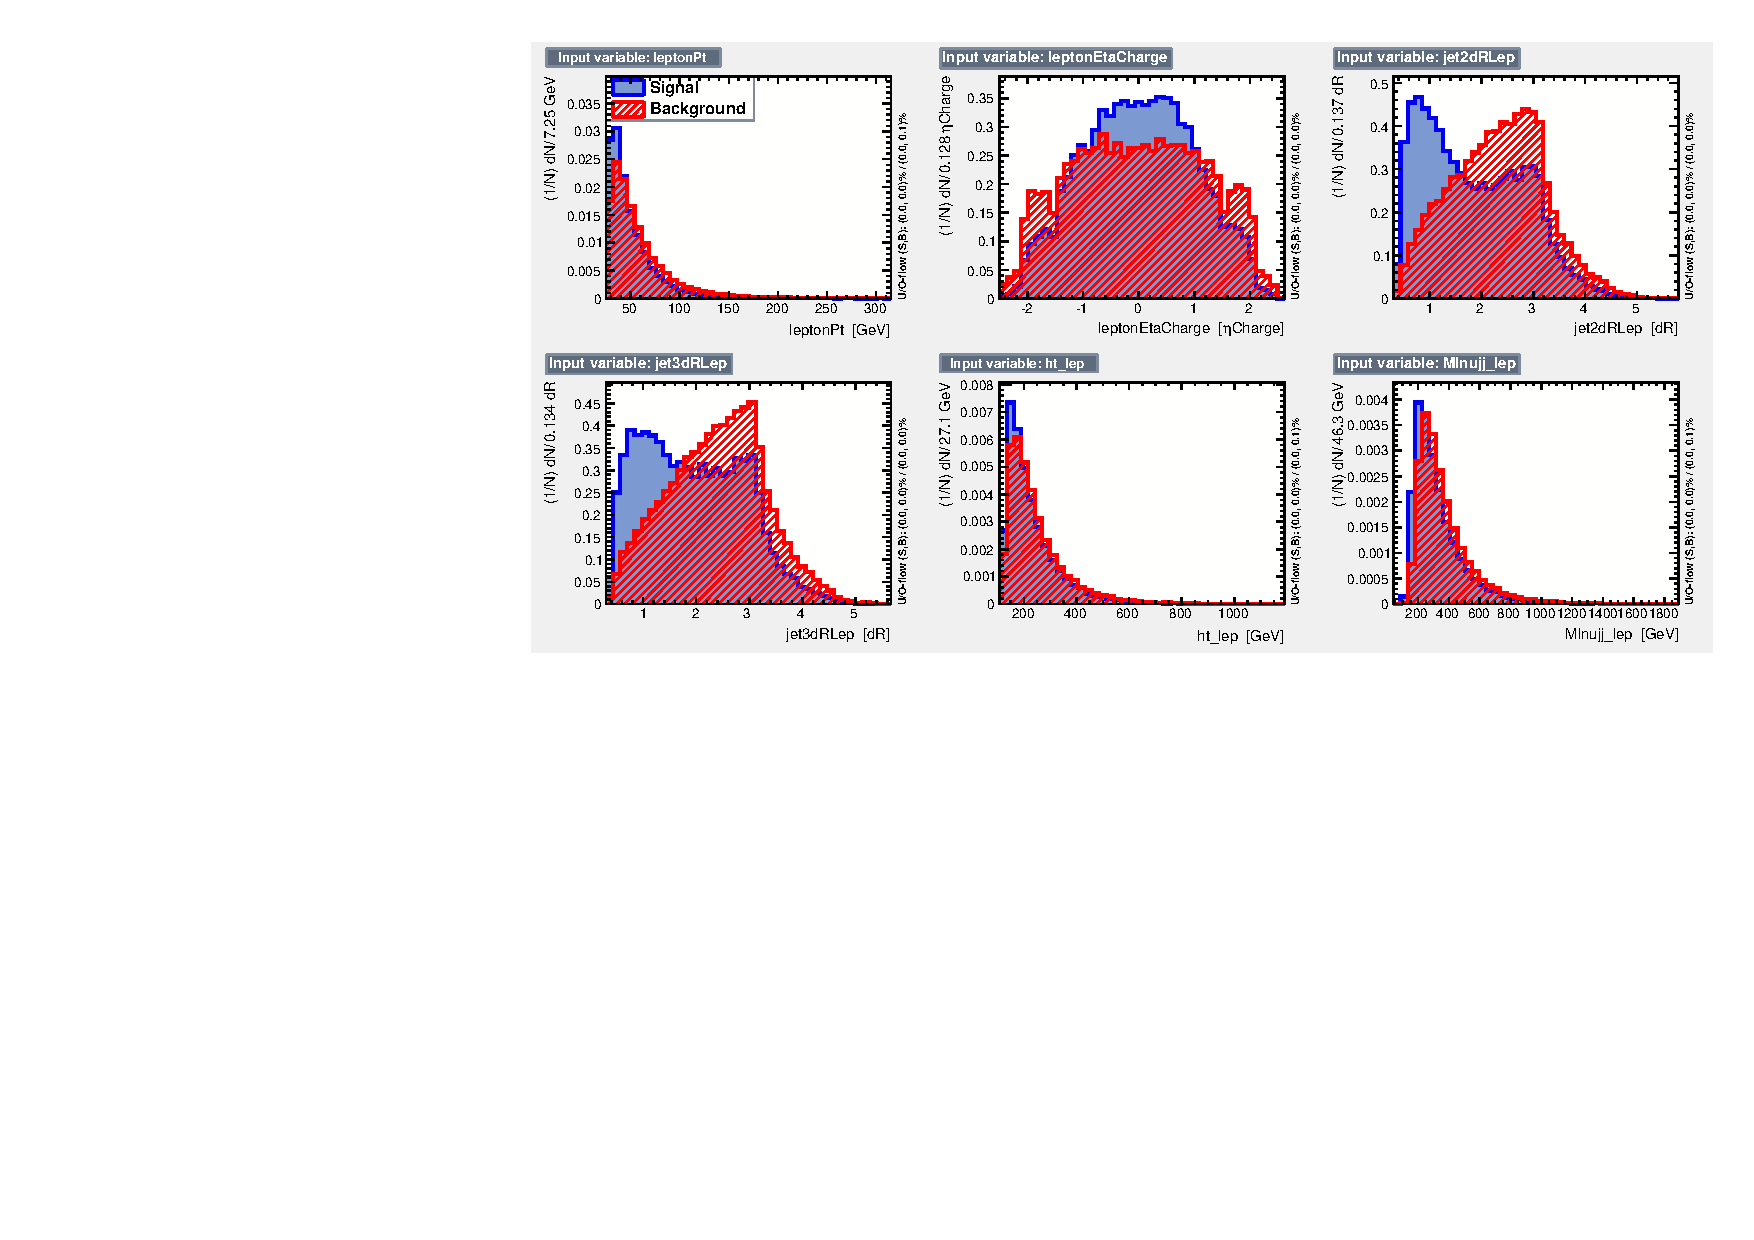
\includegraphics[width=\textwidth]{\figpath/MVA/2015_07_17_TMVA_output_jets2_eq0tag_both_HToWW_WJets_noEvtProbs_11KinVar/variables_id_c1.pdf}\\
			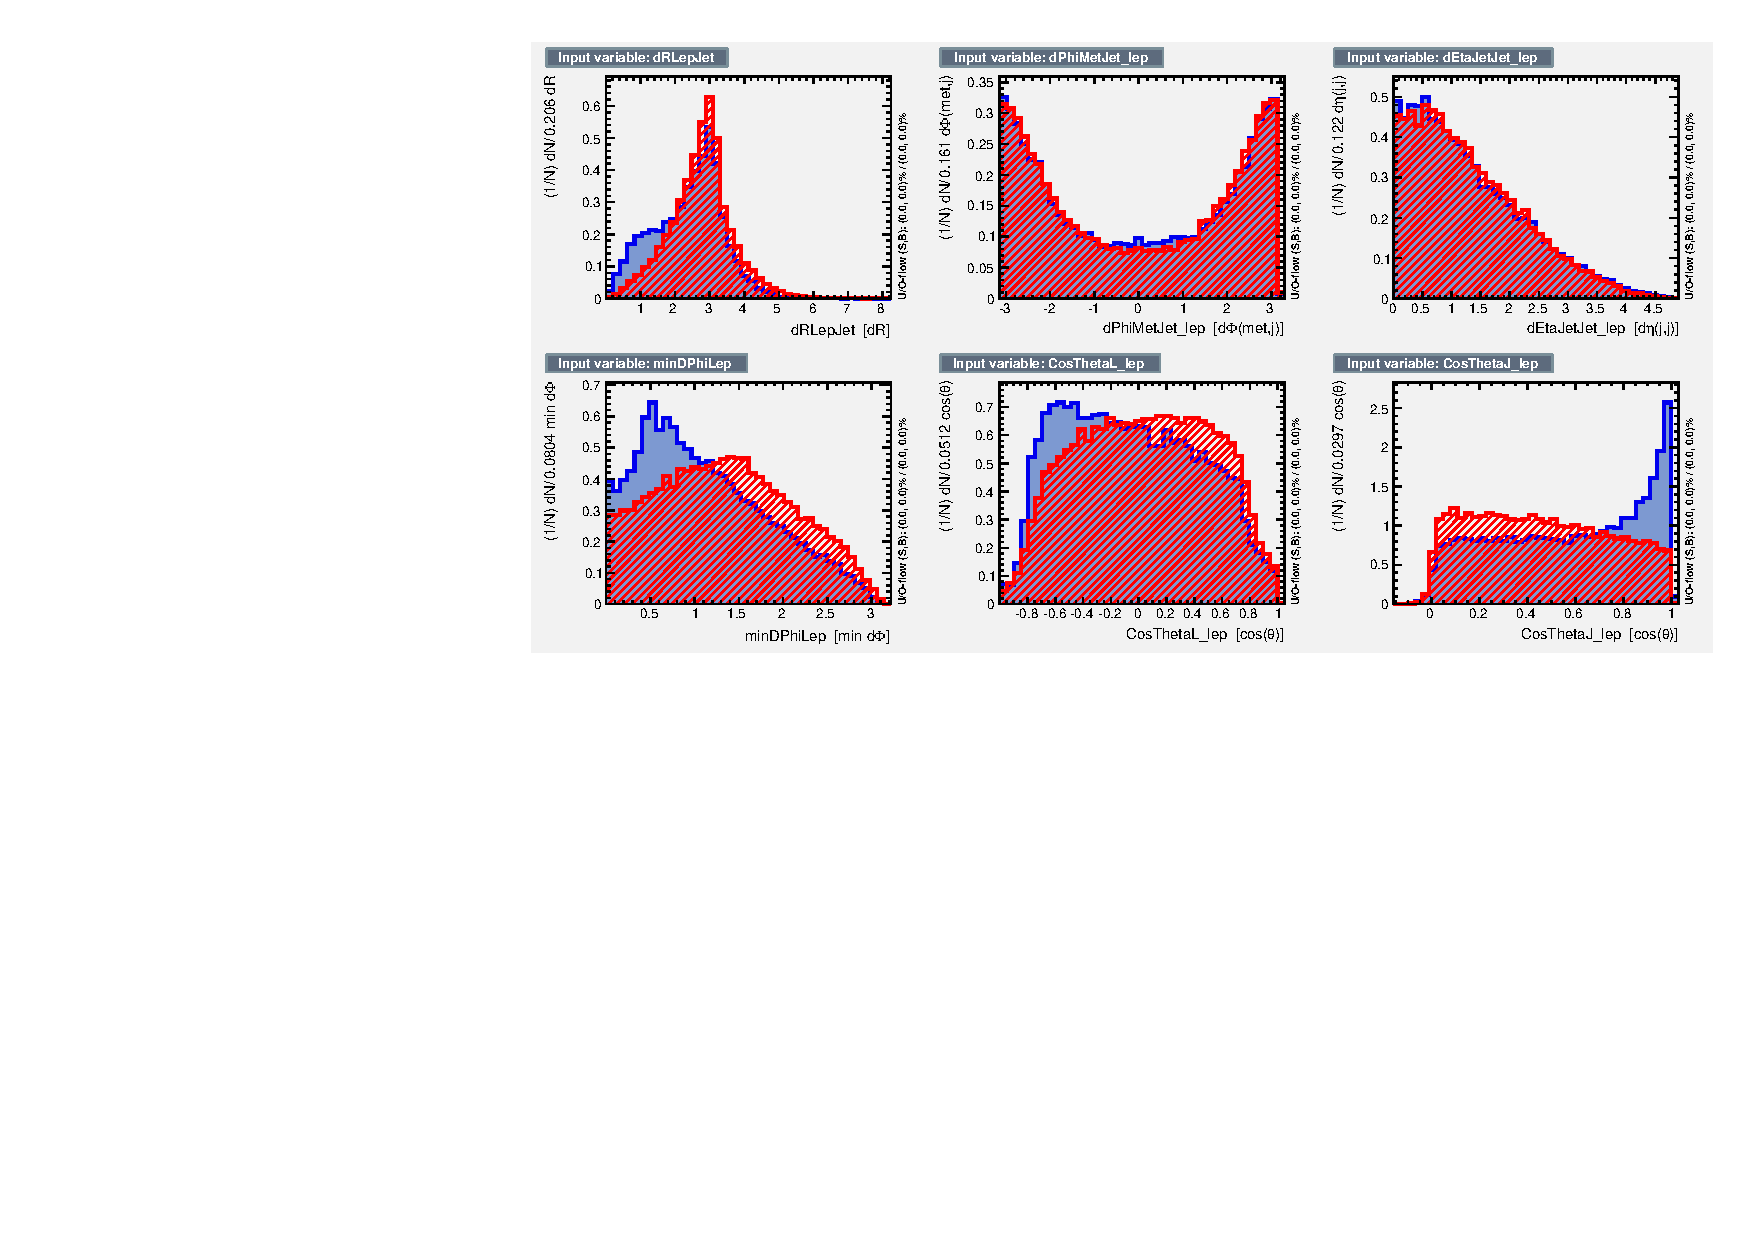
\includegraphics[width=\textwidth]{\figpath/MVA/2015_07_17_TMVA_output_jets2_eq0tag_both_HToWW_WJets_noEvtProbs_11KinVar/variables_id_c2.pdf}%
			\begin{textblock}{0.15}(0.82,0.71)
				\includegraphics[width=\textwidth]{\figpath/MVA/2015_07_17_TMVA_output_jets2_eq0tag_both_HToWW_WJets_noEvtProbs_11KinVar/mva_BDT.pdf}%
			\end{textblock}
		\end{column}
	\end{columns}
\end{frame}

%%--------------------------------------------------------------------------------------------

%\subsection*{Validation}

%%--------------------------------------------------------------------------------------------
\begin{comment}
\begin{frame}
	\frametitle{Validation of Input Variables}
	\framesubtitle{2 Jets - Electron Bin}
	\vspace*{-0.5cm}
	\begin{columns}[T]
		\column{0.31\textwidth}
			\begin{block}{\scriptsize ${\Delta}R(Jet_{2},lep)$}
				\includegraphics[width=\textwidth]{\figpath/KinematicVariables/Modified/jet2dRLep_electron.pdf}%
			\end{block}
			\vspace*{-0.15cm}
			\begin{block}{\scriptsize $\Delta\Phi(Jet_{1},Jet_{2})$}
				\includegraphics[width=\textwidth]{\figpath/KinematicVariables/Modified/DeltaPhi_J1J2_electron.pdf}%
			\end{block}
		\column{0.31\textwidth}
			\begin{block}{\scriptsize $\cos(\theta_{WH})$}
				\includegraphics[width=\textwidth]{\figpath/KinematicVariables/Modified/CosTheta_WH_electron.pdf}%
			\end{block}
			\vspace*{-0.15cm}
			\begin{block}{\scriptsize $\cos(\theta_{L})$}
				\includegraphics[width=\textwidth]{\figpath/KinematicVariables/Modified/CosTheta_l_electron.pdf}%
			\end{block}
		\column{0.31\textwidth}
			\begin{block}{\scriptsize ME BDT}
				\includegraphics[width=\textwidth]{\figpath/KinematicVariables/Modified/MEBDT_electron.pdf}%
			\end{block}
			\vspace*{-0.15cm}
			\begin{block}{\scriptsize $\Delta\Phi(\Em_{T},Jet_{1})$}
				\includegraphics[width=\textwidth]{\figpath/KinematicVariables/Modified/dPhiMETJet_electron.pdf}%
			\end{block}
	\end{columns}
	\begin{block}{}
		\begin{itemize}
			\item Excellent agreement between data and MC
			\item Very similar for the muon channel and other jet bins
		\end{itemize}
	\end{block}
\end{frame}
\end{comment}

\begin{frame}
	\frametitle{Validation of Input Variables}
	\framesubtitle{2 Jets - Muon Bin}
	\begin{columns}[T]
		\column{0.31\textwidth}
			\begin{block}{\scriptsize ${\Delta}R(Jet_{2},lep)$}
				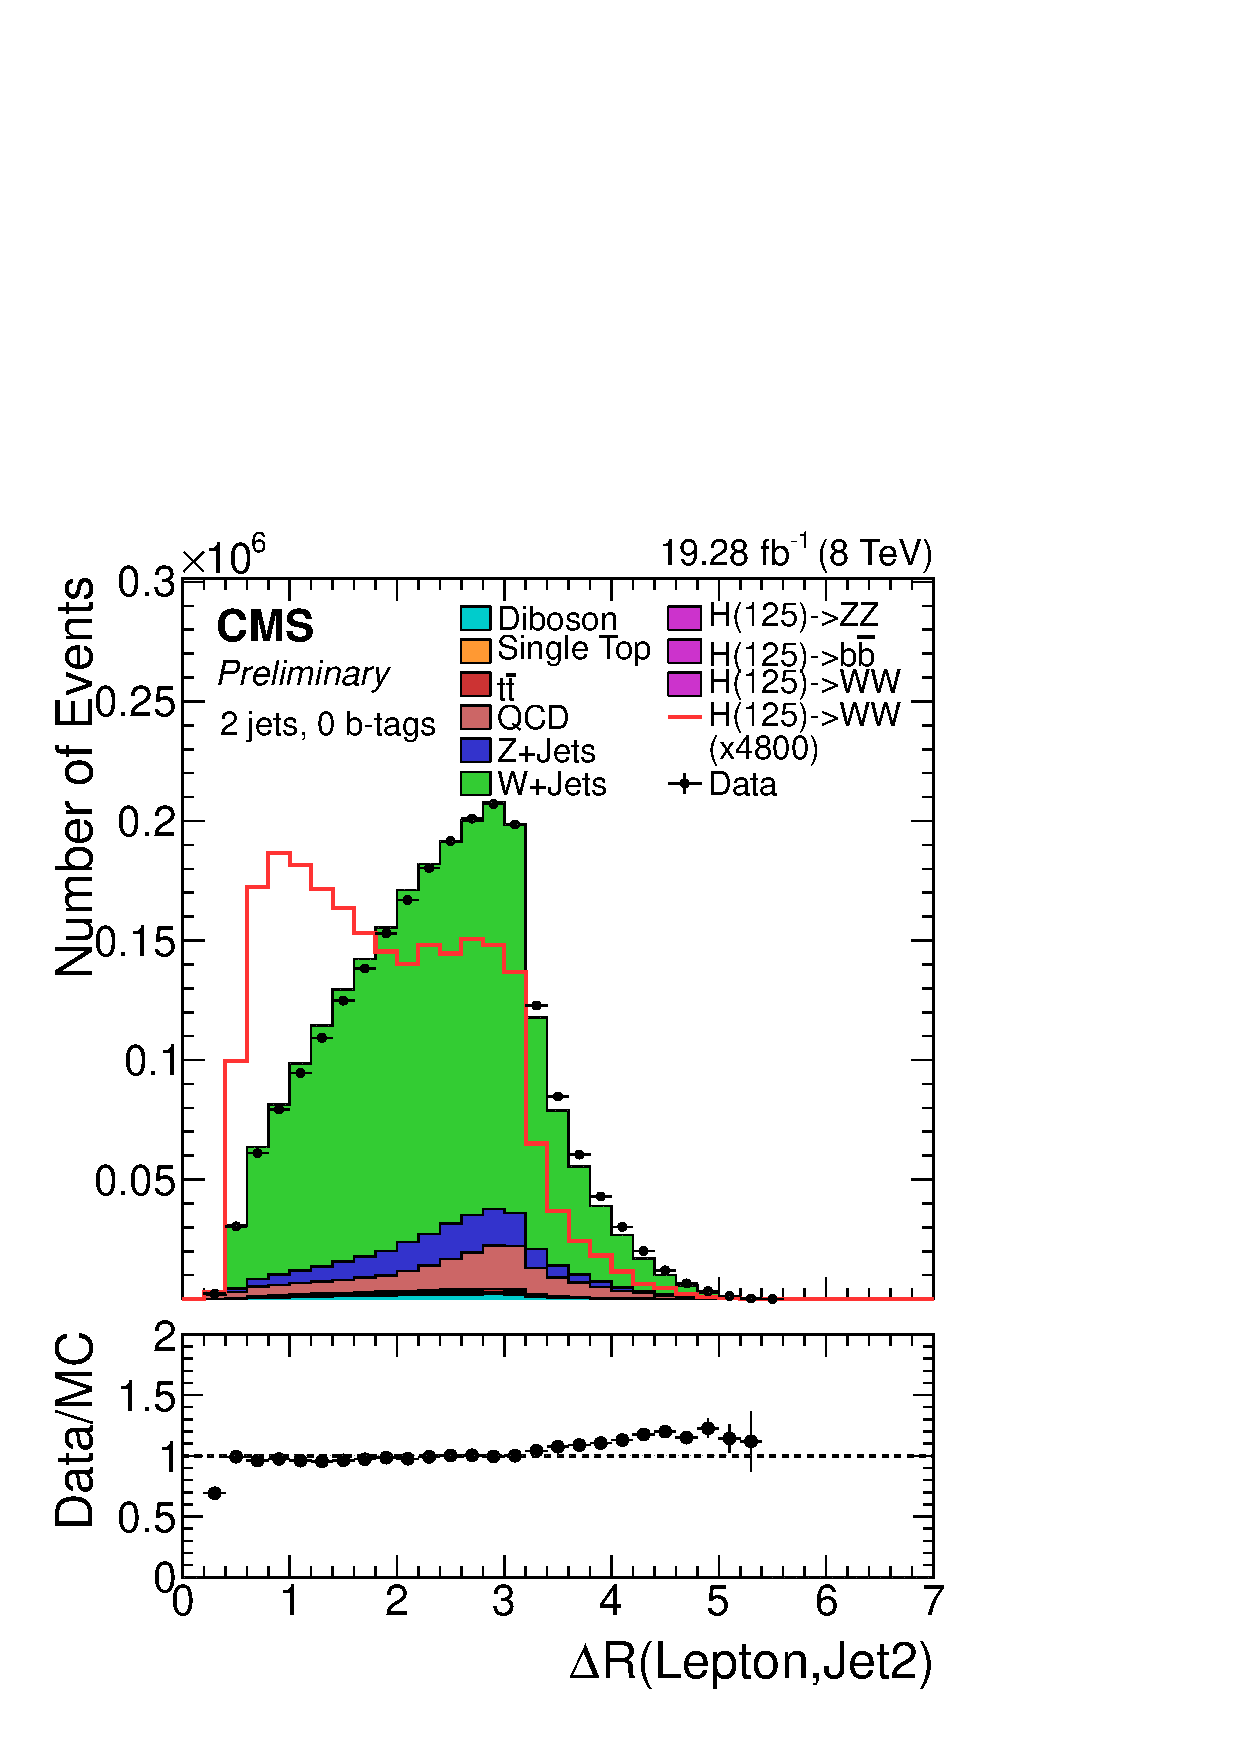
\includegraphics[width=\textwidth]{\figpath/jet2dRLep_muon_2jets.pdf}%
			\end{block}
		\column{0.31\textwidth}
			\begin{block}{\scriptsize $\cos(\theta_{L})$}
				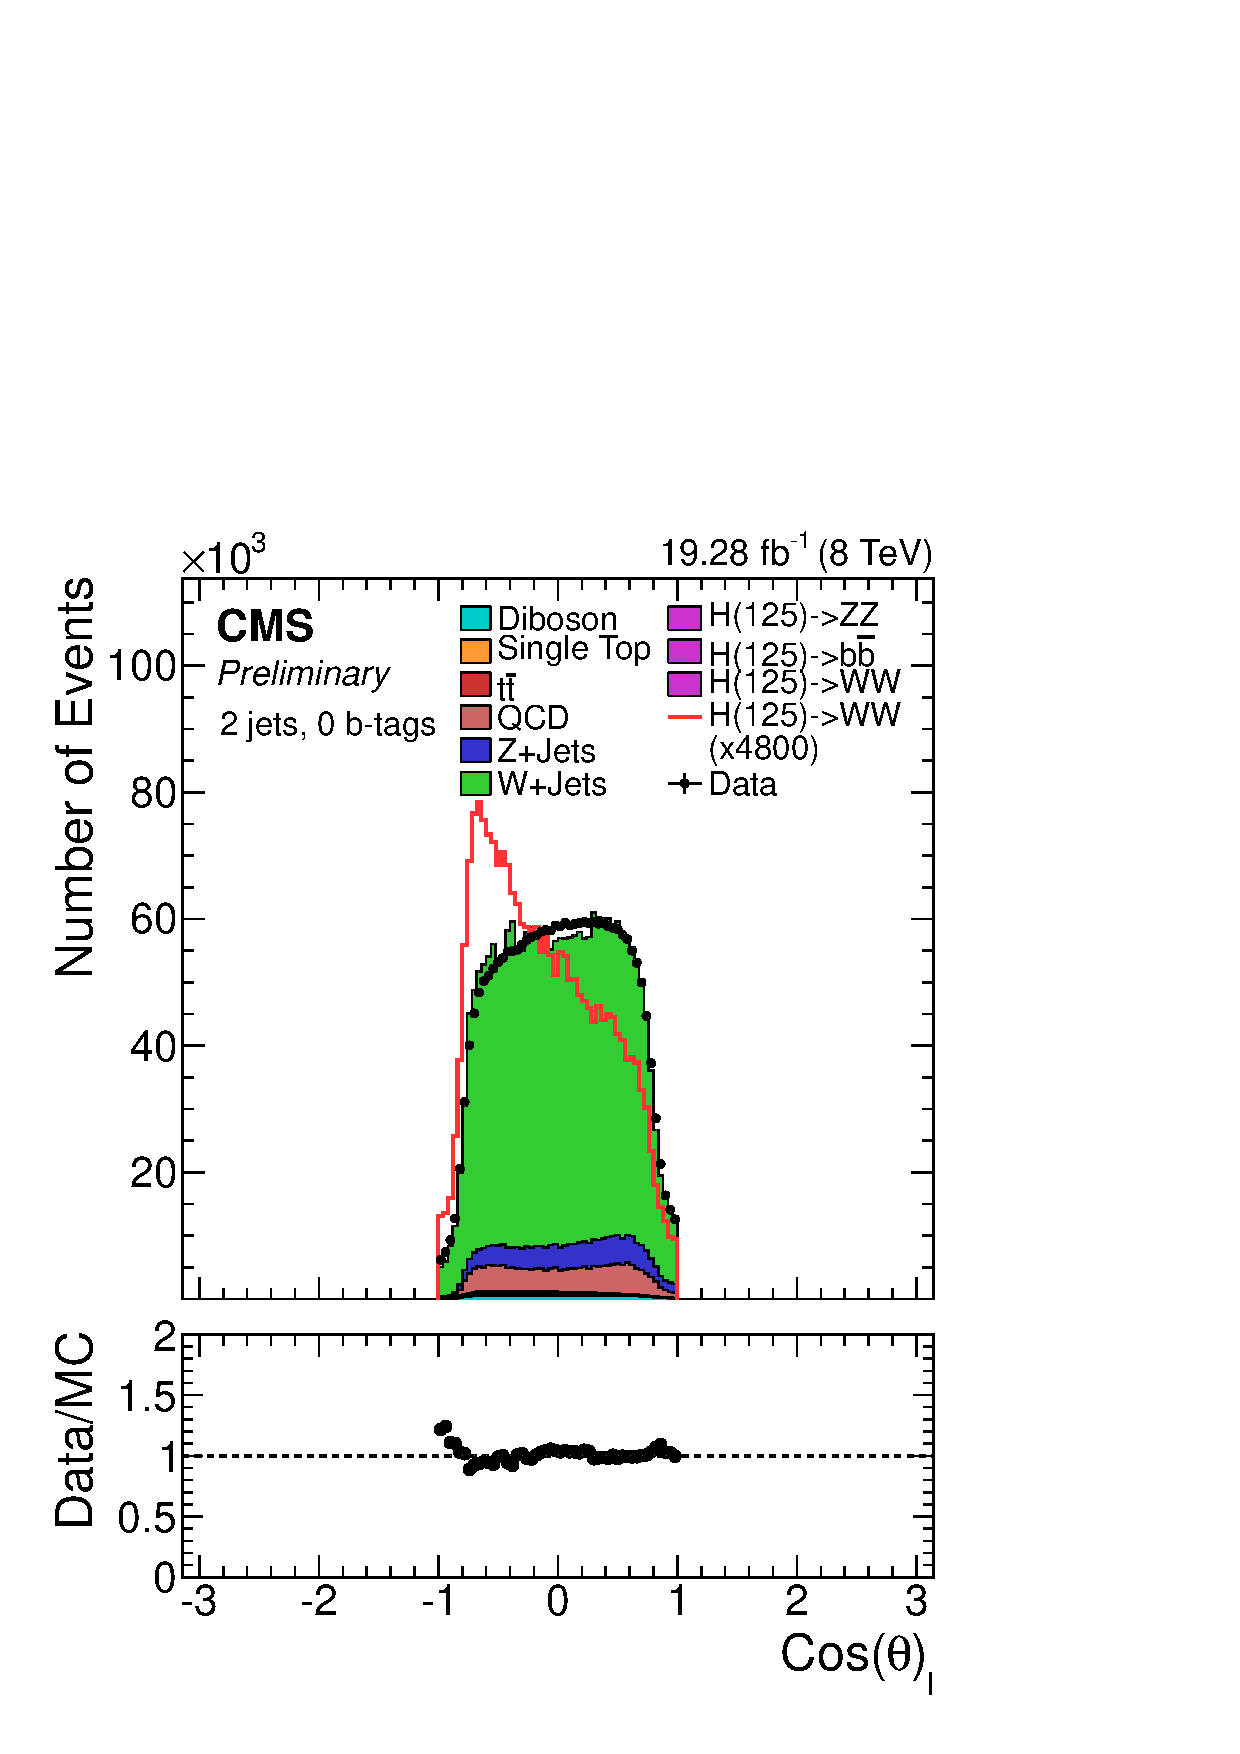
\includegraphics[width=\textwidth]{\figpath/CosTheta_l_muon_2jets.pdf}%
			\end{block}
		\column{0.31\textwidth}
			\begin{block}{\scriptsize ME BDT}
				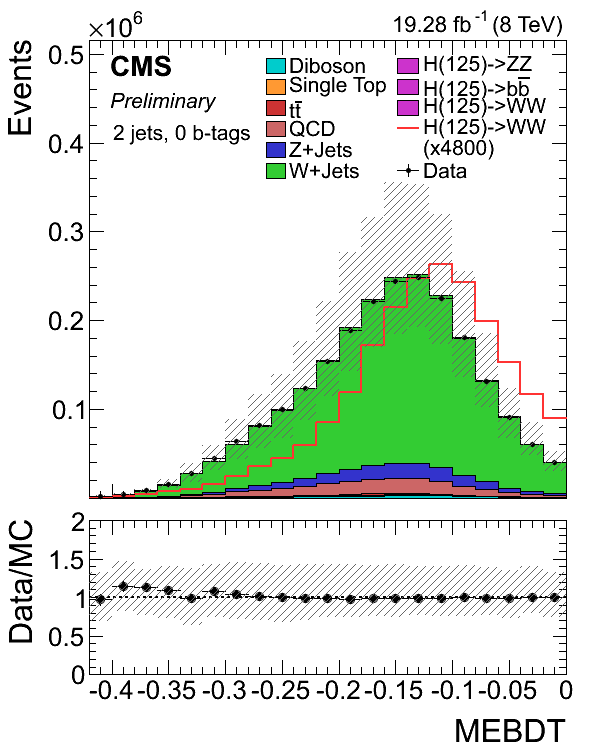
\includegraphics[width=\textwidth]{\figpath/BDTTemplates/MEBDT_jets2_muon.png}%
			\end{block}
	\end{columns}
	\begin{block}{}
		\begin{itemize}
			\item Good agreement between data and MC
			\item Very similar for the electron channel and other jet bins
		\end{itemize}
	\end{block}
\end{frame}

%%--------------------------------------------------------------------------------------------

\subsection*{Final Discriminant}

%%--------------------------------------------------------------------------------------------

\begin{frame}
	\frametitle{Matrix Element Analysis}
	\framesubtitle{Final Discriminant}
	\vspace*{-0.24cm}
		\begin{textblock}{0.96}(0.0175,0.14)
			\begin{block}{}
				\begin{itemize}
					\item BDT discriminant computed for individual jet bins
					\begin{itemize}
						\item {\color{blue}Blue: Signal}
						\item {\color{red}Red: Background}
					\end{itemize}
				\end{itemize}
			\end{block}
		\end{textblock}
		\begin{textblock}{0.96}(0.0175,0.37)
			\begin{alertblock}{BDT Discriminants}
				\centering
				\includegraphics[width=0.33\textwidth]{\figpath/MVA/2015_07_17_TMVA_output_jets2_eq0tag_both_HToWW_WJets_noEvtProbs_12KinVar/mva_BDT.pdf}%
				\includegraphics[width=0.33\textwidth]{\figpath/MVA/2015_07_17_TMVA_output_jets3_eq0tag_both_HToWW_WJets_noEvtProbs_14KinVar/mva_BDT.pdf}%
				\includegraphics[width=0.33\textwidth]{\figpath/MVA/2015_07_17_TMVA_output_jets4_eq0tag_both_HToWW_WJets_noEvtProbs_8KinVar/mva_BDT.pdf}%
			\end{alertblock}
		\end{textblock}
		\begin{textblock}{0.15}(0.24,0.53){\color{red}{2 Jets}}\end{textblock}
		\begin{textblock}{0.15}(0.56,0.53){\color{red}{3 Jets}}\end{textblock}
		\begin{textblock}{0.15}(0.88,0.53){\color{red}{$\geq$4 Jets}}\end{textblock}
		\begin{textblock}{0.96}(0.0175,0.85)
			\begin{block}{}
				\begin{itemize}
					\item Improved discrimination between signal and background!
				\end{itemize}
			\end{block}
		\end{textblock}
\end{frame}